\section{Fides \& Network Access}
\label{sec:fides-and-network-access}

\begin{figure}[ht]
    \centering
    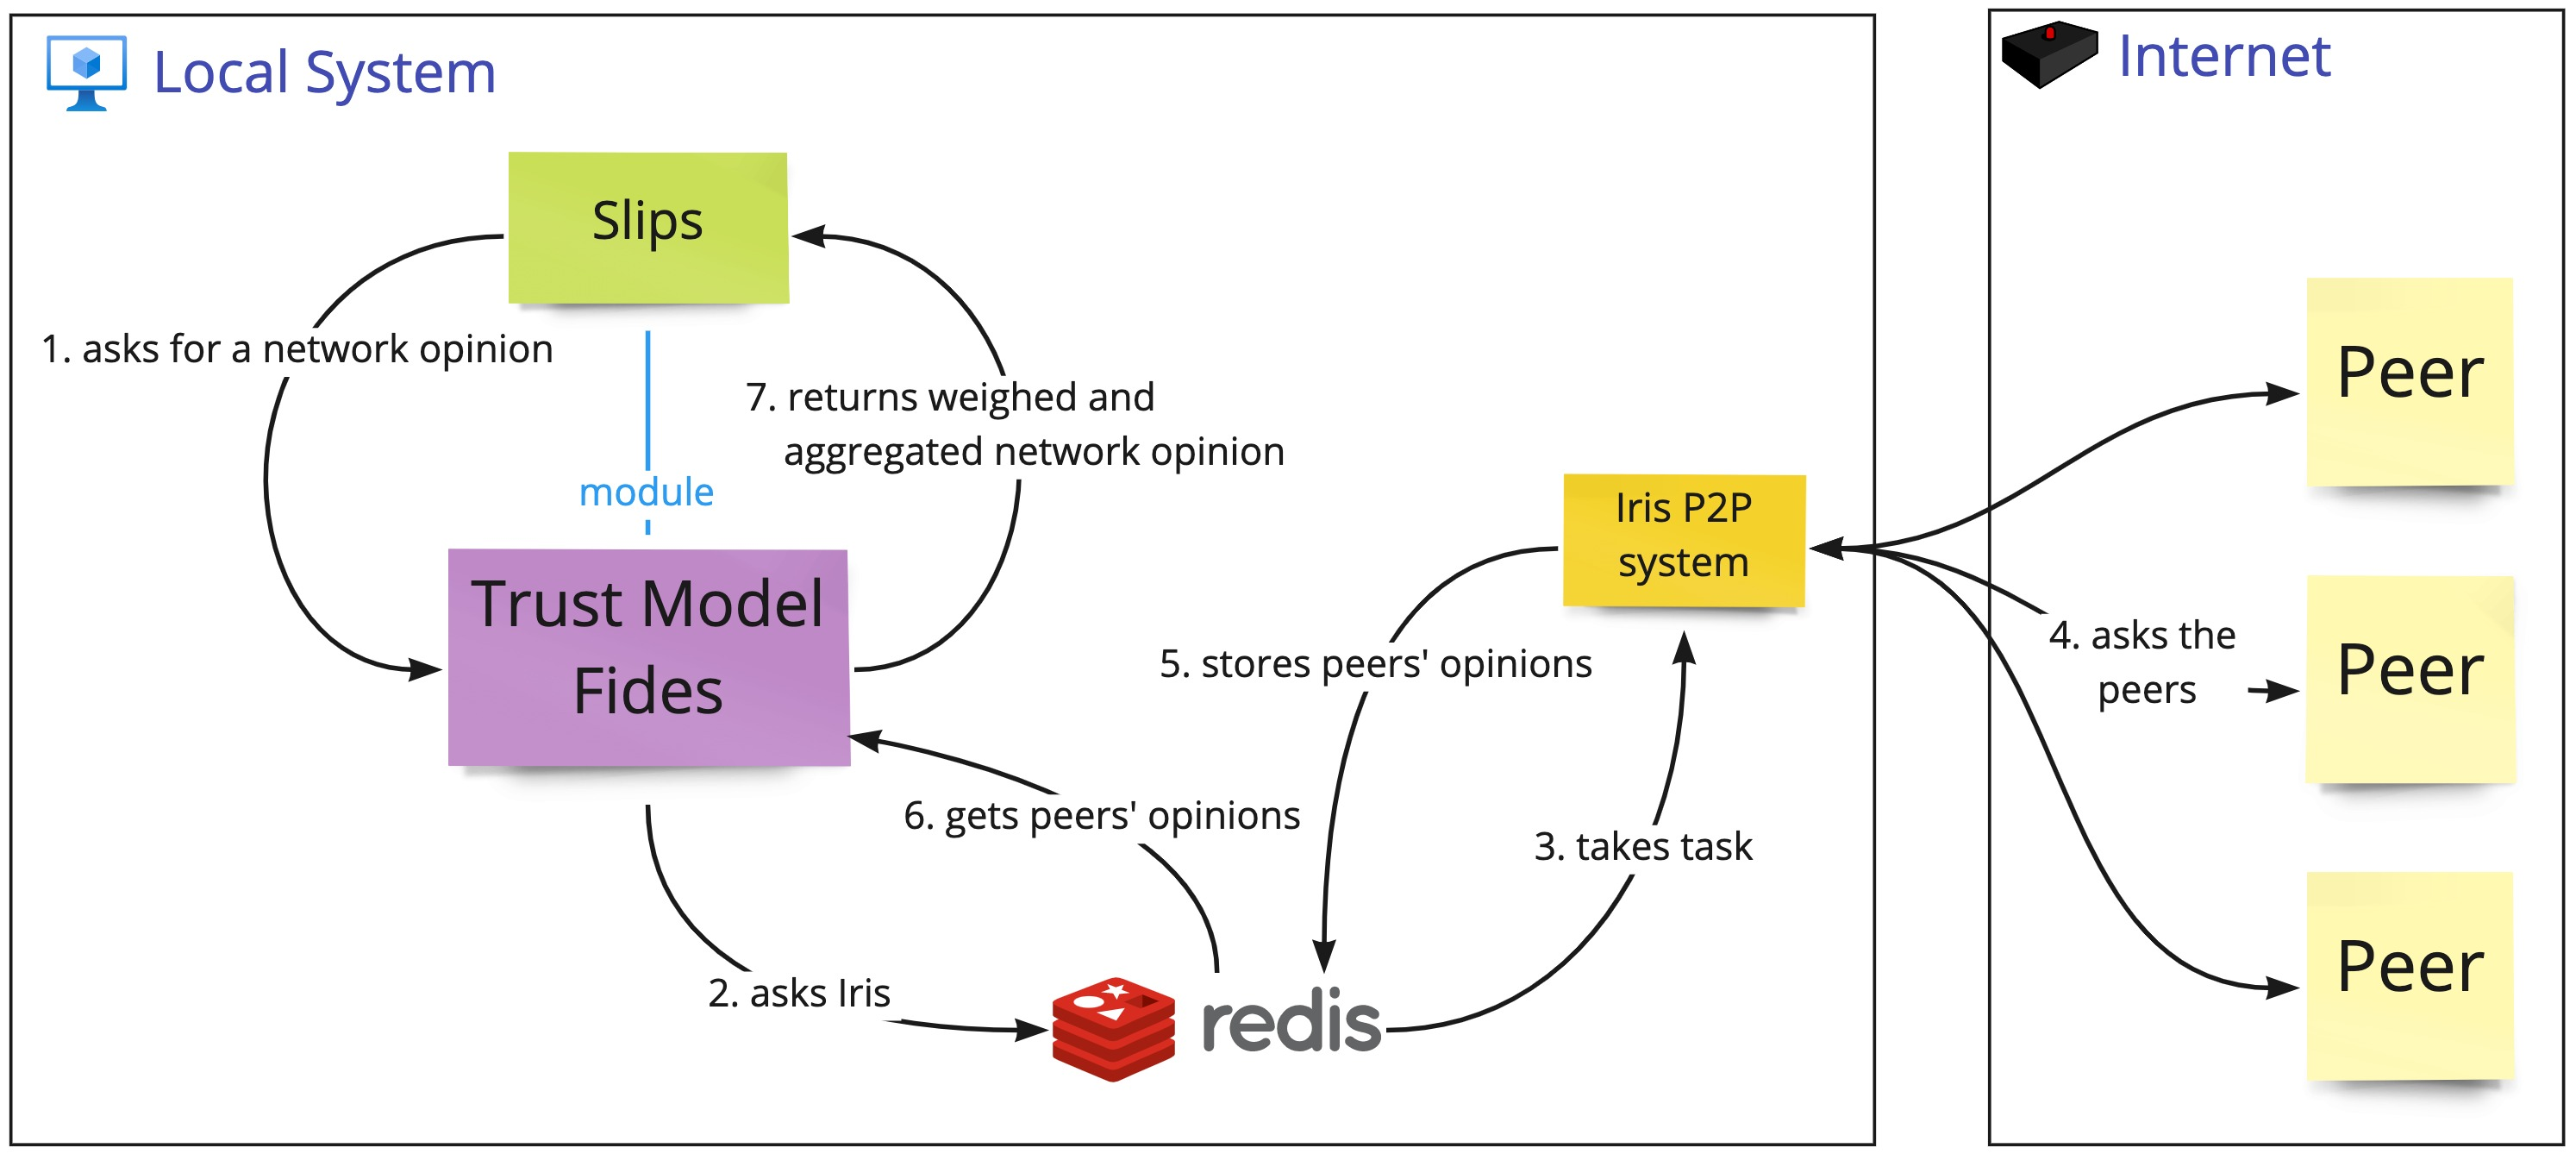
\includegraphics[width=1.0\textwidth]{assets/communication_architecture.jpeg}
    \caption{High-level overview of communication between Fides, Iris and Slips including examples of messages that sends to each other.}
    \label{fig:fides-api-network}
\end{figure}

Fides itself is a trust model and it does not interact with the network directly, but rather it exposes an API that can be used either to receive the information from the network or for sending the requests back to the network.
Thanks to this design, where all business logic is separated from the network layer, Fides is highly modular and does not depend on the network layer implementation.
The network layer Iris then performs all data transfers and facilitates all communications with the remote peers.
It also facilitates finding new peers and ensuring that all requests from Fides are dispatched to the correct recipients.
In the eyes of Fides, the network layer is a \textit{black box} and it does not need to know how the network layer is implemented.
See Figure~\ref{fig:fides-api-network} for a high-level overview of the communication.

The network layer, \textbf{Iris}, was developed by Bc. Martin Řepa in~\cite{nl} where Řepa describes how Iris works in detail and what protocols are used to safely deliver necessary information and messages between the instances of Fides.